\chapter{Resonance Compensation Studies at the CERN Proton Synchrotron Booster}
\label{sec:ch5}

\section{General Description}
The Proton Synchrotron Booster (PSB) is the first circular accelerator in the CERN accelerator complex that ultimately leads to the LHC. Figure \ref{fig:cernac} shows the entire chain of accelerators at CERN, feeding a variety of physics experiments \cite{cernplot}. Following the successful implementation of the LHC Injectors Upgrade (LIU) \cite{liu}, the PSB receives $H^-$ ion beam coming from the Linac4 at an energy of 160 MeV. Interestingly enough, the PSB is not just one ring, but rather four synchrotron rings stacked on top of each other. This is to counteract space charge effects which are largest at low energy machines. Once the ion beam enters the PSB rings, the electrons are stripped off with a carbon foil and proton beam is achieved \cite{psbstrip}. The proton beam is then accelerated from an energy of 160 MeV to 2 GeV. The beam from the four rings gets merged together and then gets injected to the Proton Synchrotron (PS). This is true for LHC-type beams, nevertheless, the PSB can also accelerate lead ions and deliver to other customers like the heavy ion experiments like ISOLDE \cite{foteini1}.   \cite{foteini2} 

\begin{figure}[H]
    \centering
    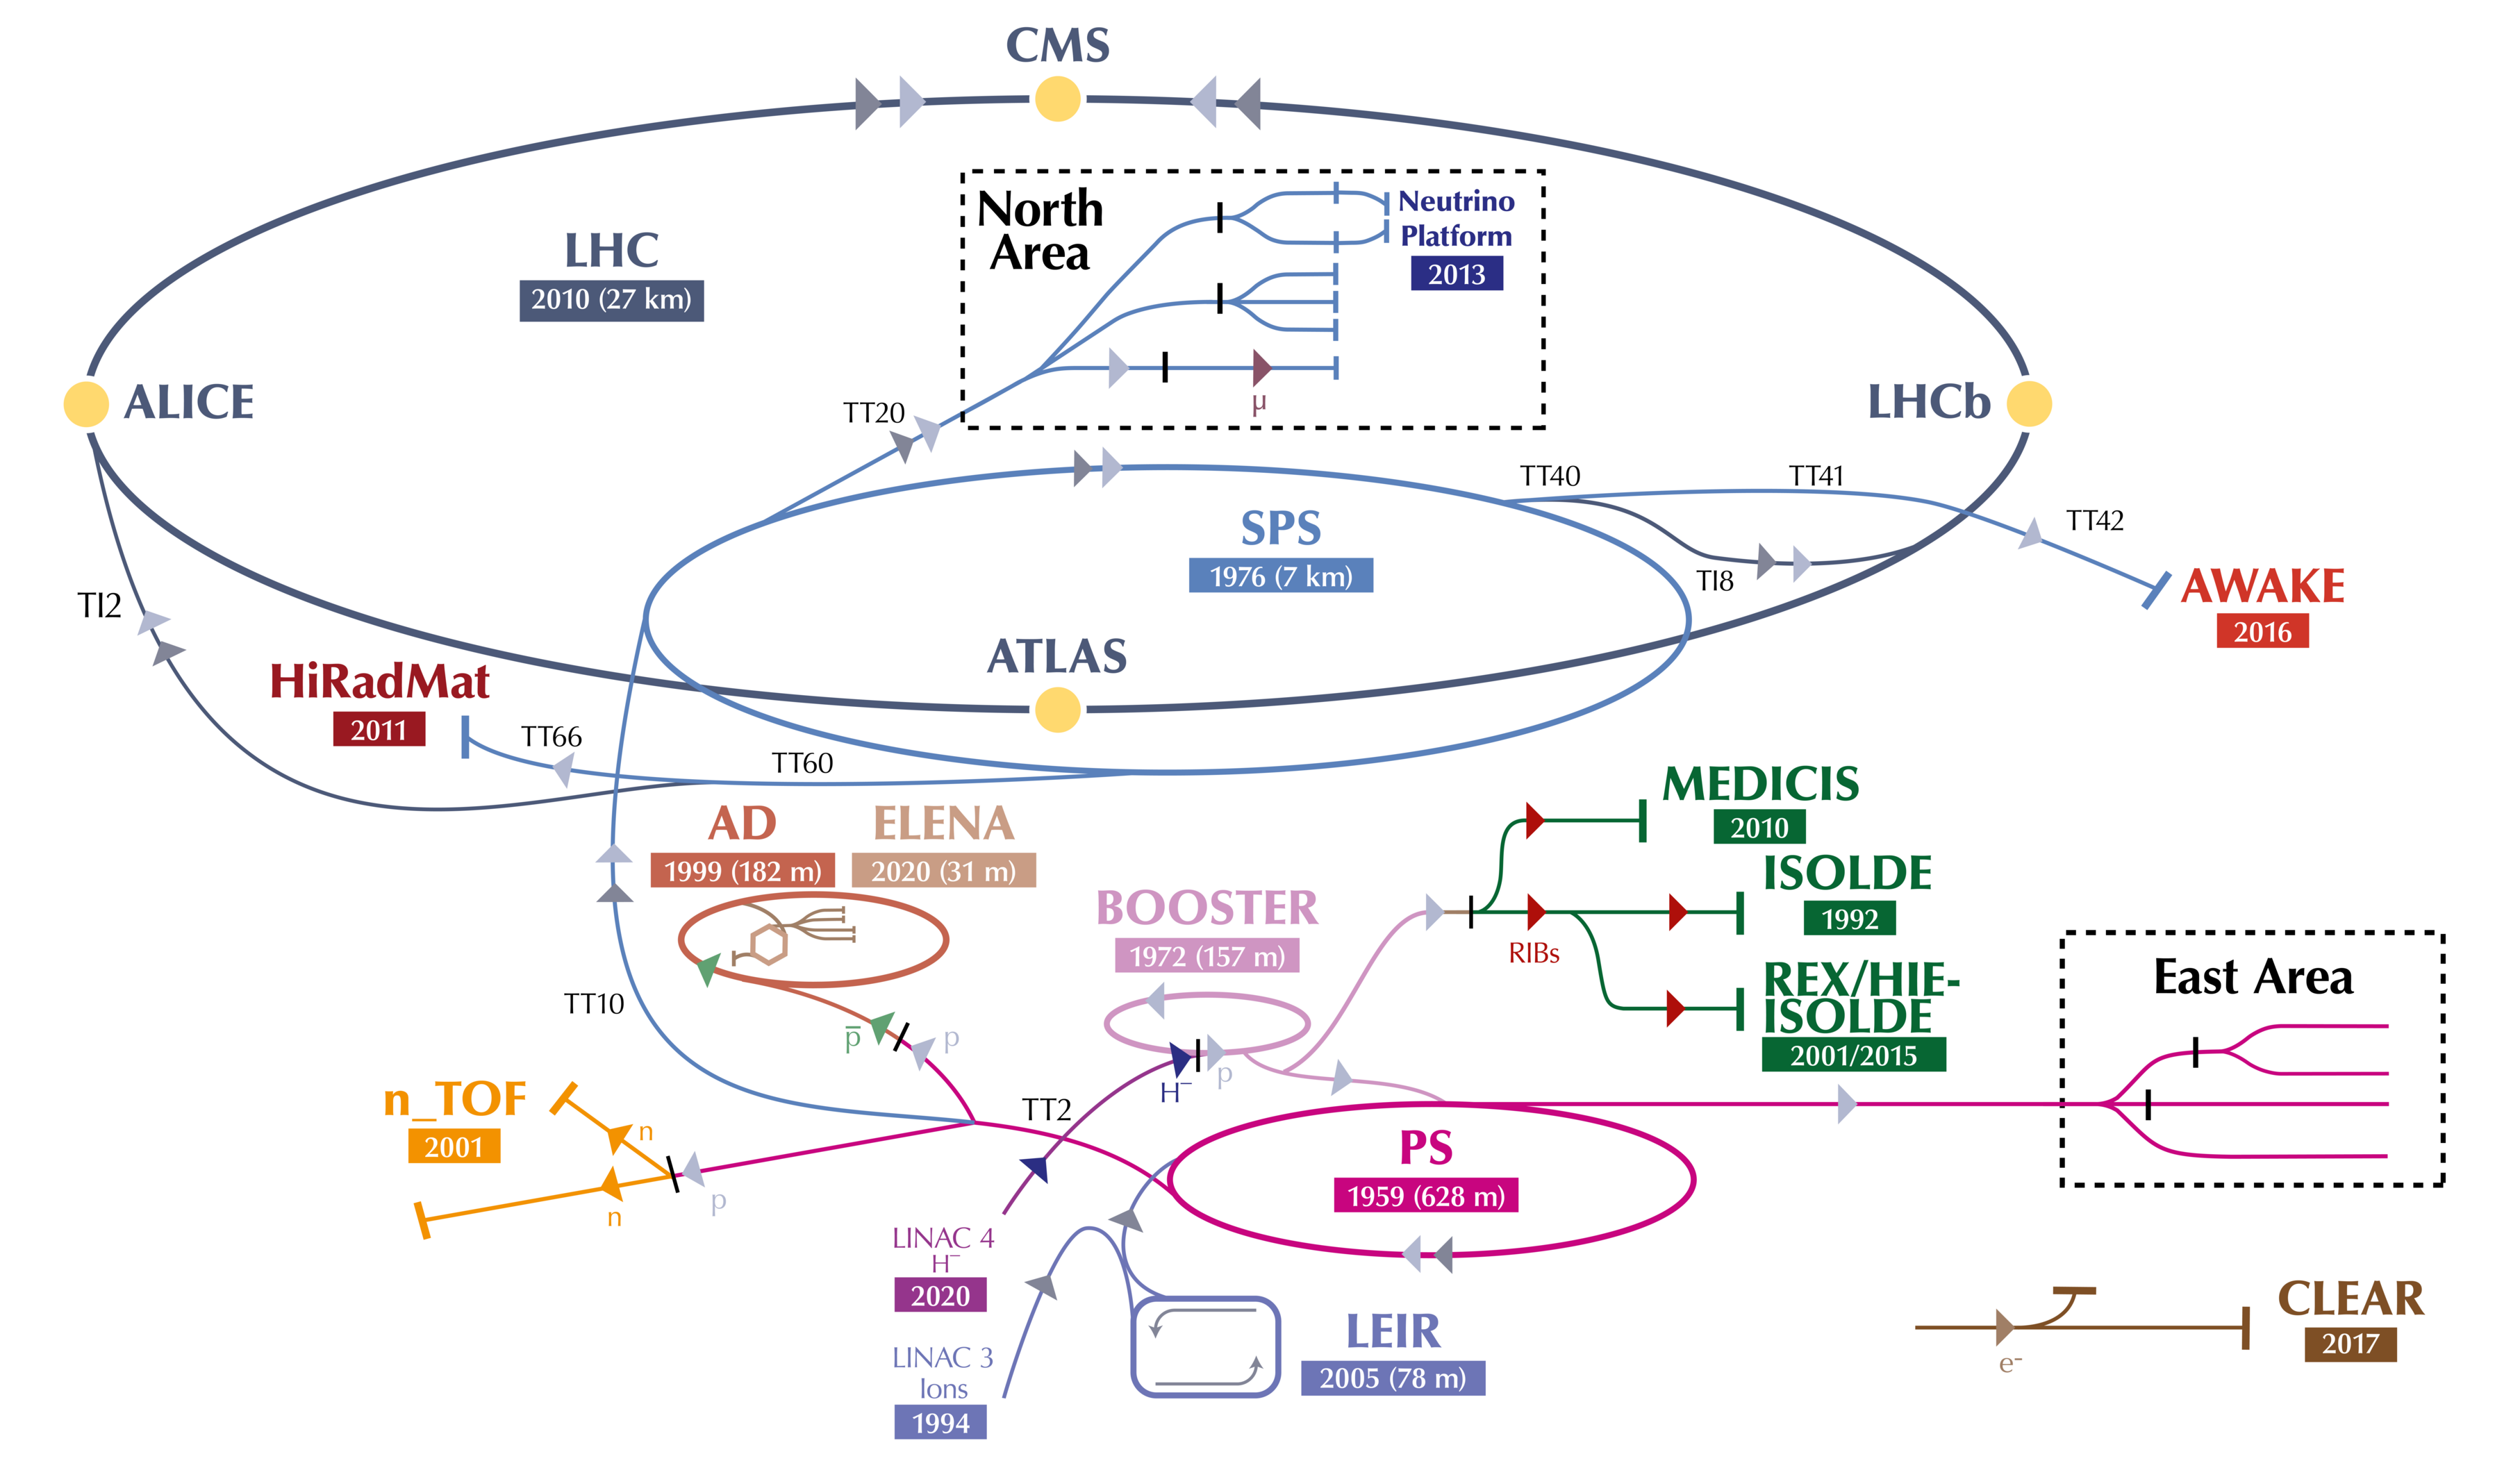
\includegraphics[width=\linewidth]{chapter5/CERN_AC.png}
    \caption{A graphic overview of all accelerators in operation at CERN as of 2022. Original image taken from Ref. \cite{cernplot}. This file is licensed under the Creative Commons Attribution 4.0 International license.}
    \label{fig:cernac}
 \end{figure}

\section{Tune Diagram and Operation}

\section{Optimization Algorithms for Resonance Compensation}

\section{Experimental Verification of Compensation}
